\documentclass[xcolor=x11names,compress,professionalfonts, aspectratio=169]{beamer}

%% General packages %%%%%%%%%%%%%%%%%%%%%%%%%%%%%%%%%%
\usepackage[utf8]{inputenc}
\usepackage{graphicx}
\usepackage{tikz}
\tikzset{% change default arrow tips
    >=latex
}
\usepackage{ifthen}

\usepackage{amsmath}
\usepackage{nicefrac}

\usepackage{color}

% compile child documents using this preamble
\usepackage{subfiles}

% compile child files with separate preambles, and include them in the document
\usepackage{standalone}

%%%%%%%%%%%%%%%%%%%%%%%%%%%%%%%%%%%%%%%%%%%%%%%%%%%%%%

\makeatletter
\setbeamertemplate{footline}
{
    \leavevmode%
    \hbox{%
        \begin{beamercolorbox}[wd=.333333\paperwidth,ht=2.25ex,dp=1ex,center]{author in head/foot}%
            \usebeamerfont{author in head/foot}\insertshortauthor
        \end{beamercolorbox}%
                \begin{beamercolorbox}[wd=.333333\paperwidth,ht=2.25ex,dp=1ex,center]{title in head/foot}%
            \usebeamerfont{title in head/foot}\insertshorttitle
        \end{beamercolorbox}%
        \begin{beamercolorbox}[wd=.333333\paperwidth,ht=2.25ex,dp=1ex,right]{date in head/foot}%
            \usebeamerfont{date in head/foot}\insertshortdate{}\hspace*{2em}
            \insertframenumber{} / \inserttotalframenumber\hspace*{2ex} 
        \end{beamercolorbox}}%
        \vskip0pt%
    }
    \makeatother


%% Beamer Layout %%%%%%%%%%%%%%%%%%%%%%%%%%%%%%%%%%
\useoutertheme[subsection=false,shadow]{miniframes}
\useinnertheme{rectangles}

\setbeamertemplate{navigation symbols}{}%remove navigation symbols

\author{Nicolas Macé}

\newcommand{\btVFill}{\vskip0pt plus 1filll}%place an element at the bottom of the page

\usepackage{libertine}
\usepackage[T1]{fontenc}

\setbeamerfont{title like}{shape=\scshape}
\setbeamerfont{frametitle}{shape=\scshape}

\setbeamercolor*{lower separation line head}{bg=DeepSkyBlue4} 
\setbeamercolor*{normal text}{fg=black,bg=white} 
\setbeamercolor*{alerted text}{fg=red} 
\setbeamercolor*{example text}{fg=black} 
\setbeamercolor*{structure}{fg=black} 
 
\setbeamercolor*{palette tertiary}{fg=black,bg=black!10} 
\setbeamercolor*{palette quaternary}{fg=black,bg=black!10} 

\renewcommand{\(}{\begin{columns}}
\renewcommand{\)}{\end{columns}}
\newcommand{\<}[1]{\begin{column}{#1}}
\renewcommand{\>}{\end{column}}

\definecolor{BostonBlue}{HTML}{00688B}
\definecolor{Complementary}{HTML}{8B2300}

% letters A and B appearing in the qp chains
\newcommand{\A}{\textcolor{BostonBlue}{A}}
\newcommand{\B}{\textcolor{Complementary}{B}}

\renewcommand{\ss}[1]{\scriptsize{\text{#1}}}
%%%%%%%%%%%%%%%%%%%%%%%%%%%%%%%%%%%%%%%%%%%%%%%%%%

\usepackage{braket}
% compile child documents using this preamble
\usepackage{subfiles}

%%%My Math

\newcommand{\pd}[2]{\frac{\displaystyle \partial #1}{\displaystyle\partial #2}} % for partial derivatives
\renewcommand{\d}[1]{\mathrm{d}#1}

\begin{document}

\section{2D models: the ``grown-up example''}
\subsection{Dummy}

\begin{frame}{2D tilings}
We consider the Penrose and the Ammann-Beenker tilings.
\begin{columns}
\begin{column}{5cm}
{\centering
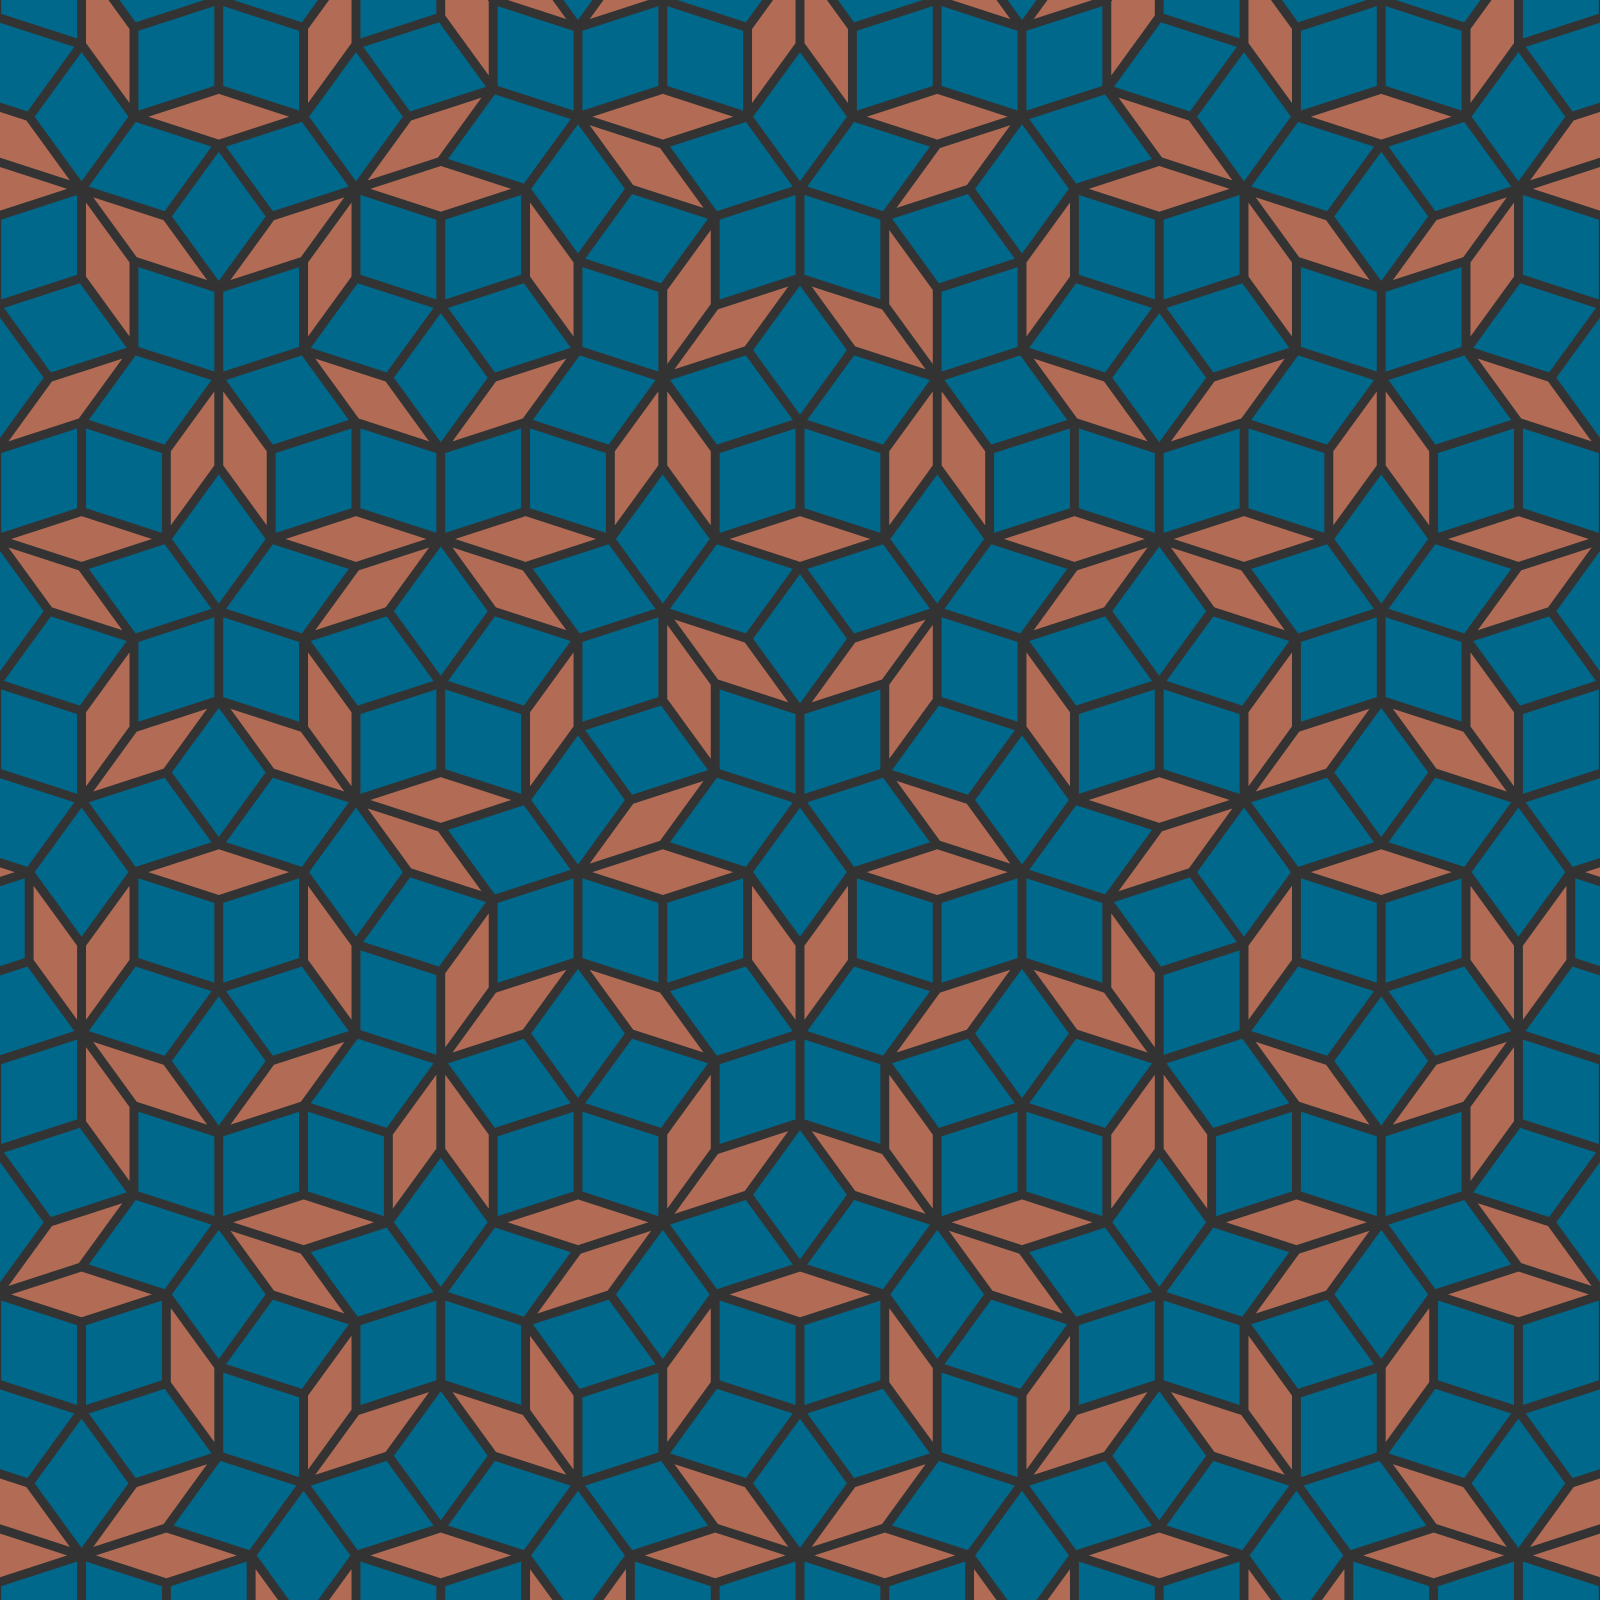
\includegraphics[scale=.09]{img/penrose.png}

}
\end{column}
\begin{column}{5cm}
{\centering
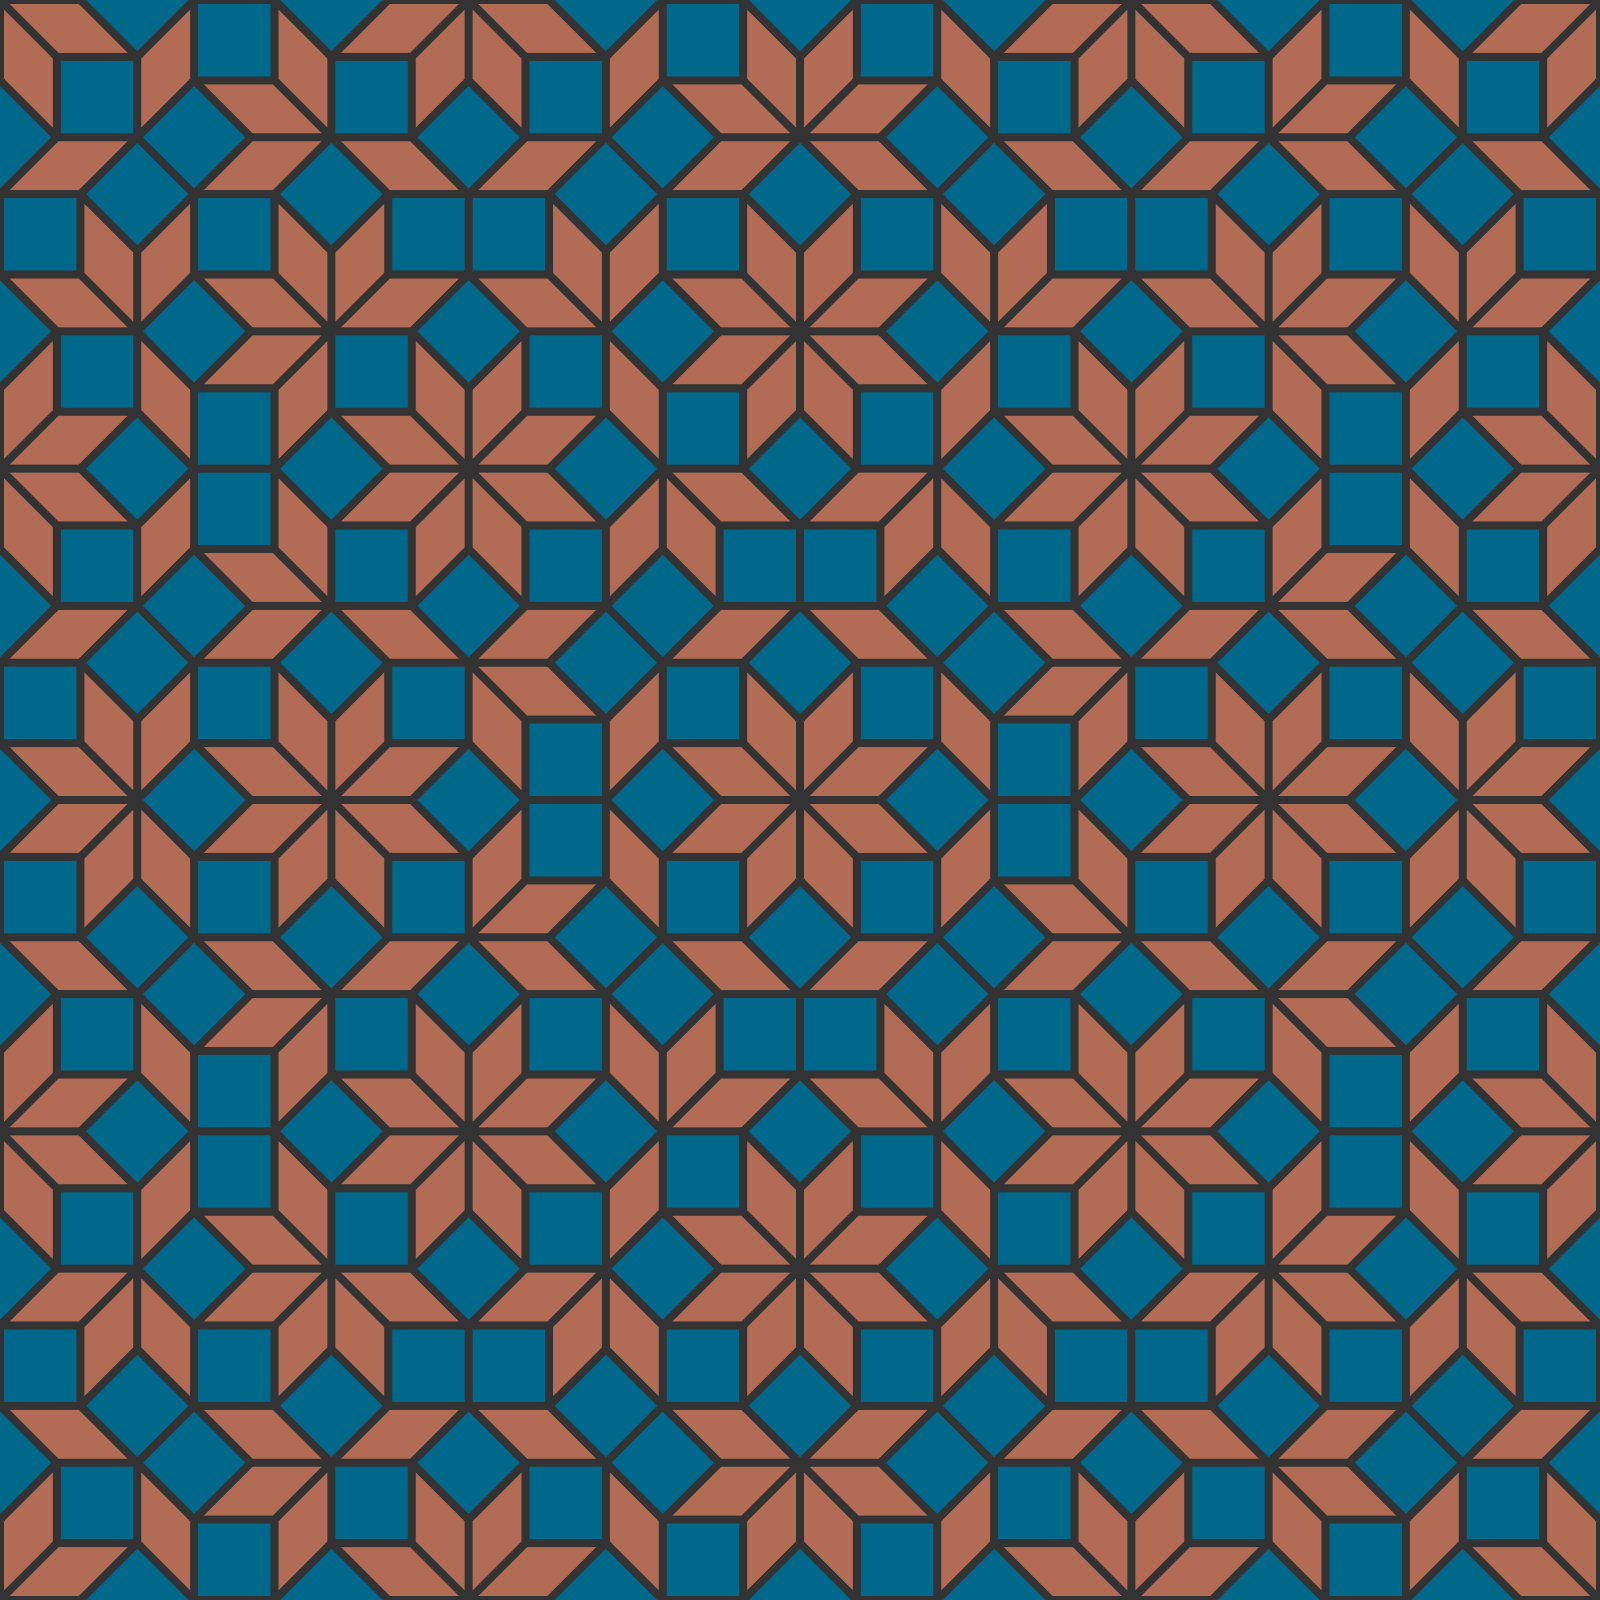
\includegraphics[scale=.09]{img/ammann-beenker.png}

}
\end{column}
\<{4cm}
Model for the electron:
\[
	E \psi_m = V_m \psi_m + t\sum_{n \in V(m)} \psi_n
\]
\>
\end{columns}

\end{frame}

\begin{frame}{What is known}

Local density of states [taken from Zijlstra 2014]:

{\centering
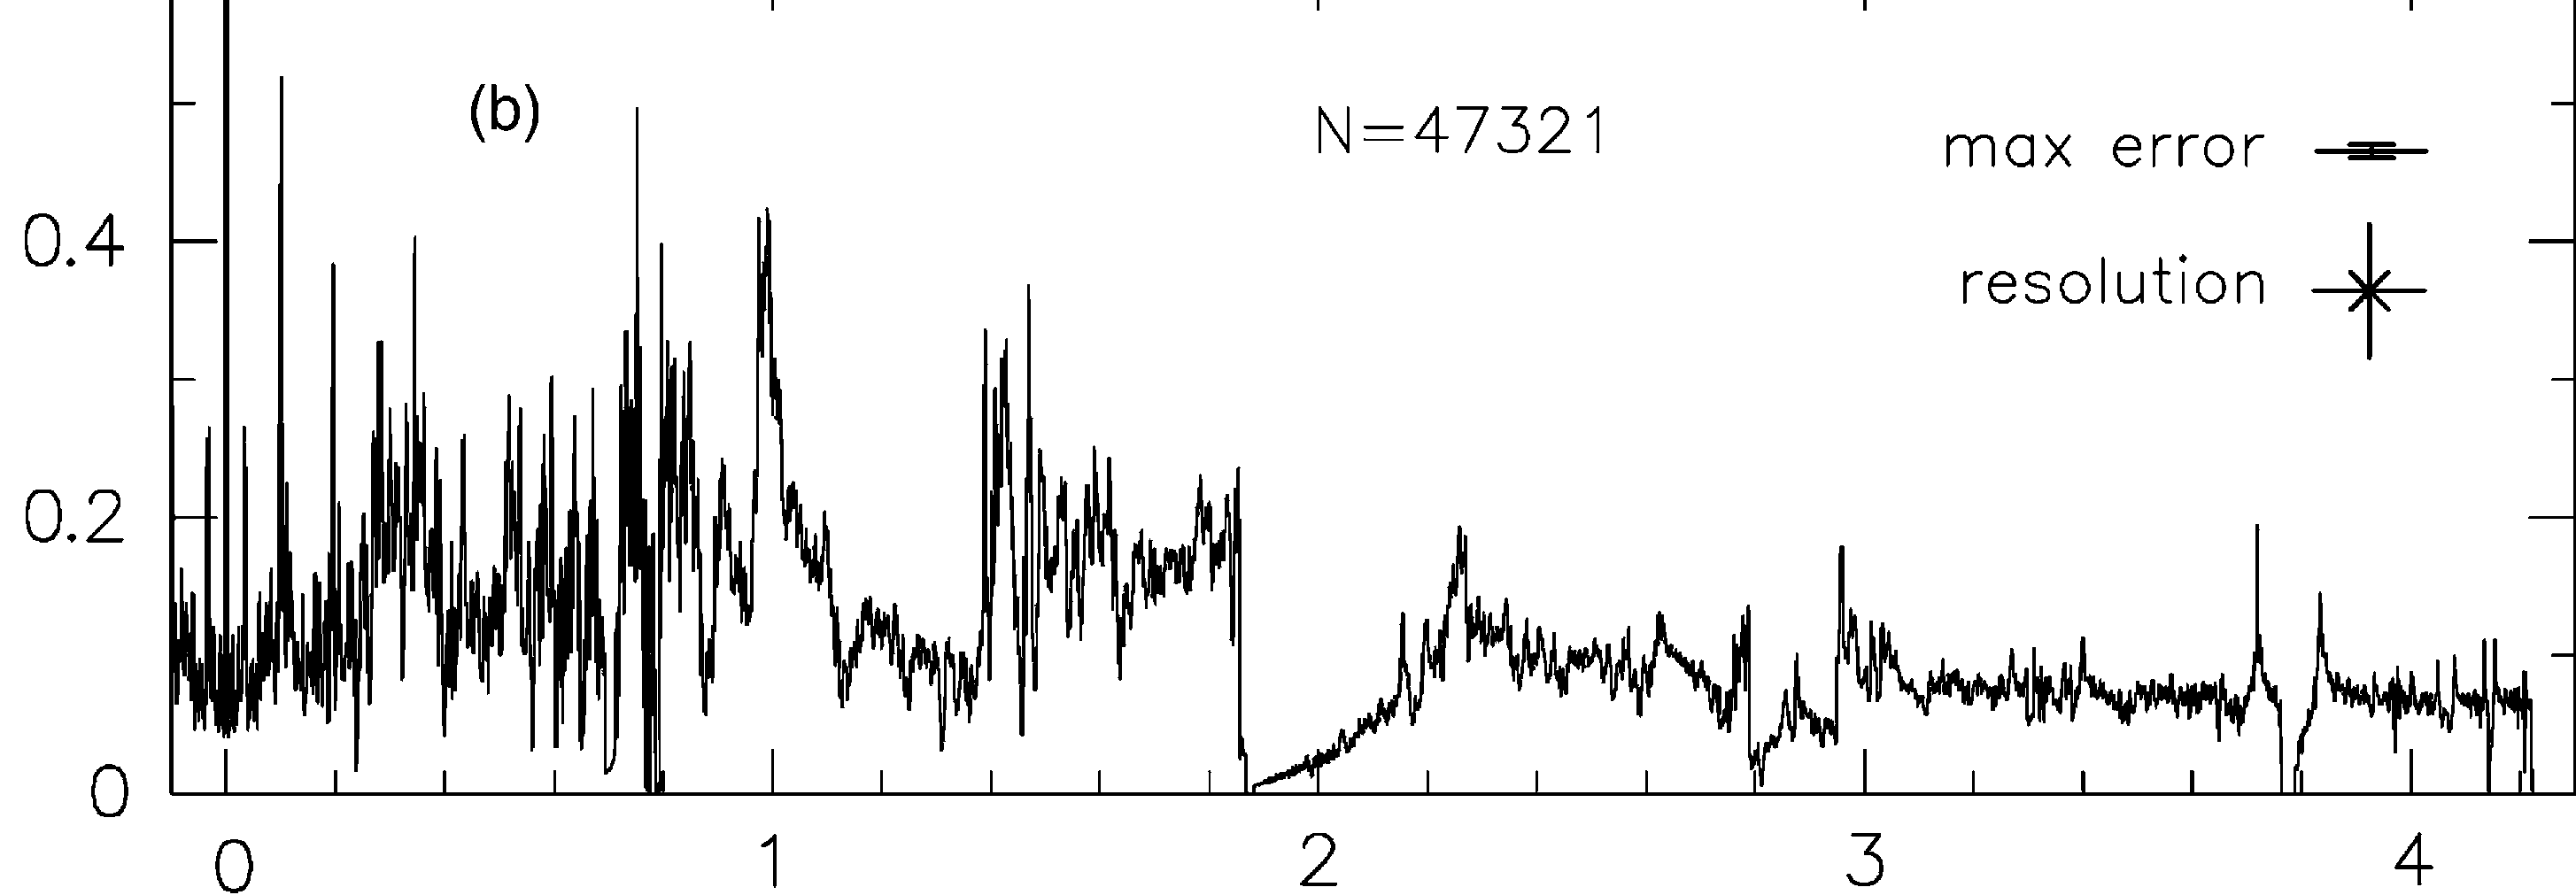
\includegraphics[scale=.1]{img/idos_AB_small.png}

}
\begin{itemize}
	\item Spectrum: no apparent fractal structure
	\item States are critical (numerical result, eg [Rieth, Schreiber 1998])
\end{itemize}
$\rightarrow$ can we introduce a field of arrows to describe some of these critical wavefunctions?
\end{frame}

\begin{frame}{A natural field of arrows}

In superspace, arrows go from the center to the border of the slice:

{\centering
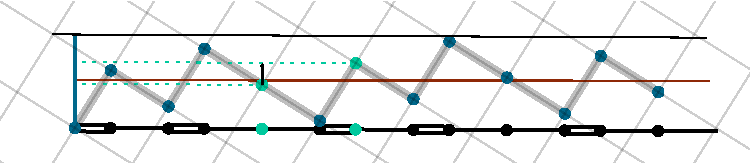
\includegraphics[scale=.8]{img/cut_and_project_arrows.pdf}

}

\begin{columns}
\<{7cm}
\begin{itemize}
	\item Define arrows in the same way for 2D tilings
	\item Consider again the height: $h(m) = \sum A$
\end{itemize}
	Can we describe states with this arrow field? $\psi_m = \rho^{h(m)}$
\>
\<{7cm}
{\centering
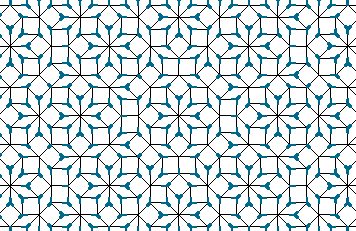
\includegraphics[scale=.9]{img/arrowed_tiling_excerpt.pdf}

}
\>
\end{columns}

\end{frame}

\begin{frame}{The groundstate wavefunction}
Can we find an ``arrowed state'' $\psi_m = \rho^{h(m)}$ ?
\begin{itemize}
\item Idea [Sutherland 1986]: tune the potential
\[
	E \psi_m = V_m \psi_m + t \sum_{n \in V(m)} \psi_n \Longleftrightarrow V_m = E - t\sum_n \beta^{A_{m,n}}
\]
Obtain a groundstate which is an arrowed state.

Not very physical! Generically, potential is not finely tuned.

\item ~[Kalugin, Katz 2014] conjecture: state still arrowed, but with a local modulation:
\[
	\psi_m = C_{m} \rho^{h(m)}
\]
where $C_m$ is local:
\[
	C_m \simeq C_n \text{~ if the tiling looks the same around $m$ and $n$}
\]
\end{itemize}
\end{frame}

\begin{frame}{Robustness of the structure}

\begin{columns}
\<{8cm}
\includegraphics[scale=.5]{img/gs.png}
\>
\<{6cm}
\begin{itemize}
\item The groundstate is \textbf{very robust}: 

For any model of the form
\[
	E \psi_m = V_m \psi_m + t\sum_{n} \psi_n
\]
the groundstate is an ``arrowed state''
\[
  \psi_m = C_m \rho^{h(m)}
\]
\item Same arguments as in 1D: the state has power law decay, and is critical.
\end{itemize}
$\rightarrow$ what can we do now?
\>
\end{columns}
\end{frame}

\begin{frame}{Scaling of the groundstate}

\begin{columns}
\<{7cm}
\begin{itemize}
	\item Participation ratio over a region $\mathcal{R}$:
	\[
		\text{PR}(\psi, \mathcal{R}) = \frac{\left( \sum_{m \in \mathcal{R}}|\psi_m|^2 \right)^2}{\left( \sum_{m\in \mathcal{R}} |\psi_m|^4 \right)^4}
	\]
	\item Scaling with the region volume $\text{Vol}(\mathcal{R})$:
	\[
		\text{PR}(\psi, \mathcal{R}) \sim \text{Vol}(\mathcal{R})^{D(\psi)}
	\]
	\begin{itemize}
		\item $D(\psi) = 0 \implies \psi$ localized
		\item $D(\psi) = 1 \implies \psi$ extended
		\item $0 < D(\psi) < 1 \implies \psi$ critical
 	\end{itemize}
\end{itemize}
\>

\<{7cm}
We can compute the scaling analytically for the groundstate:
\[
\boxed{
D(\psi) = \log\left( \frac{\omega(\rho^2)^2}{\omega(\rho^4)}\right)/\log \omega(1)
}
\]
with (for Ammann-Beenker)
\begin{align*}
\omega(z) &= \frac{a(z)+\sqrt{a(z)^2 - z^2}}{z} \\
a(z) &= 4 z^2 + 9 z + 4
\end{align*}
Scaling only depends on the arrow distribution, only on the \textbf{geometry} of the tiling.
\>
\end{columns}
\end{frame}

\begin{frame}{Conclusion}
\begin{itemize}
	\item Non-interacting eigenstates on quasicrystals are generically \textbf{critical}: here we were able to understand it for some specific states, both in 1D and 2D.
	\begin{itemize}
		\item 1D (Fibonacci): the $E=0$ state
		\item 2D (Penrose and Ammann-Beenker): the groundstate.
	\end{itemize}
	\item In our examples, wavefunction is described by a geometrical quasiperiodic function, the \textbf{field of arrows}.
	\item In 2D, this description is robust to changes in the model (varying potential, hopping)
	\item Using this description, we can easily computed physical quantities easily
\end{itemize}
Perspectives:
\begin{itemize}
	\item Test 2D quasicrystals: generalized Penrose, dodecagonal \dots
	\item For Penrose and Ammann-Beenker, the arrow field is not enough to describe excited states. What extra ingredients are required?
\end{itemize}
\end{frame}

%%%%%%%%%%%% Extra slides %%%%%%%%%%%%%
\begin{frame}{Cut and project chains are special!}
Consider the chain constructed by the substitution
\begin{align*}
	A & \to ABBB \\
	B & \to A
\end{align*}
\begin{columns}
\<{6cm}
\begin{itemize}
	\item This substitution cannot be built by cut and project (because it is non-Pisot).
	\item Height resembles a random walk, and typical height $\sim \sqrt{L}$
	\item As a result, the wavefunction is localized! 
\end{itemize}
\>
\<{6cm}
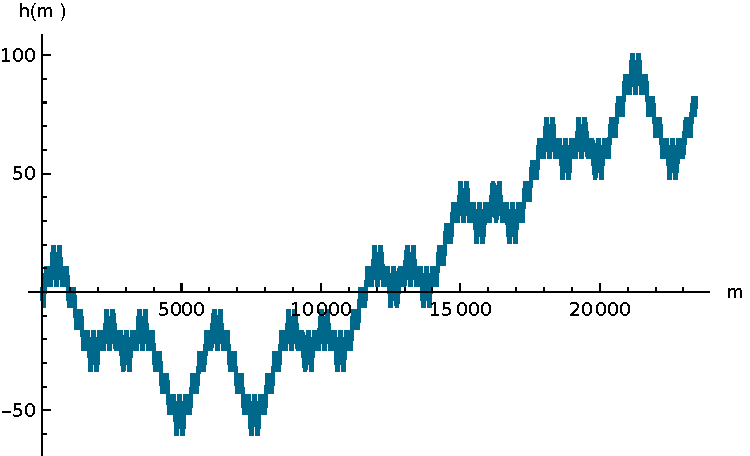
\includegraphics[scale=.5]{img/heightsB3.pdf}
\>
\end{columns}
$\rightarrow$ criticality is sensitive to the \textbf{complexity} of the tiling
\end{frame}

\begin{frame}{Theory/numerics on the 2D groundstate}
\begin{columns}
\<{7cm}
\centering
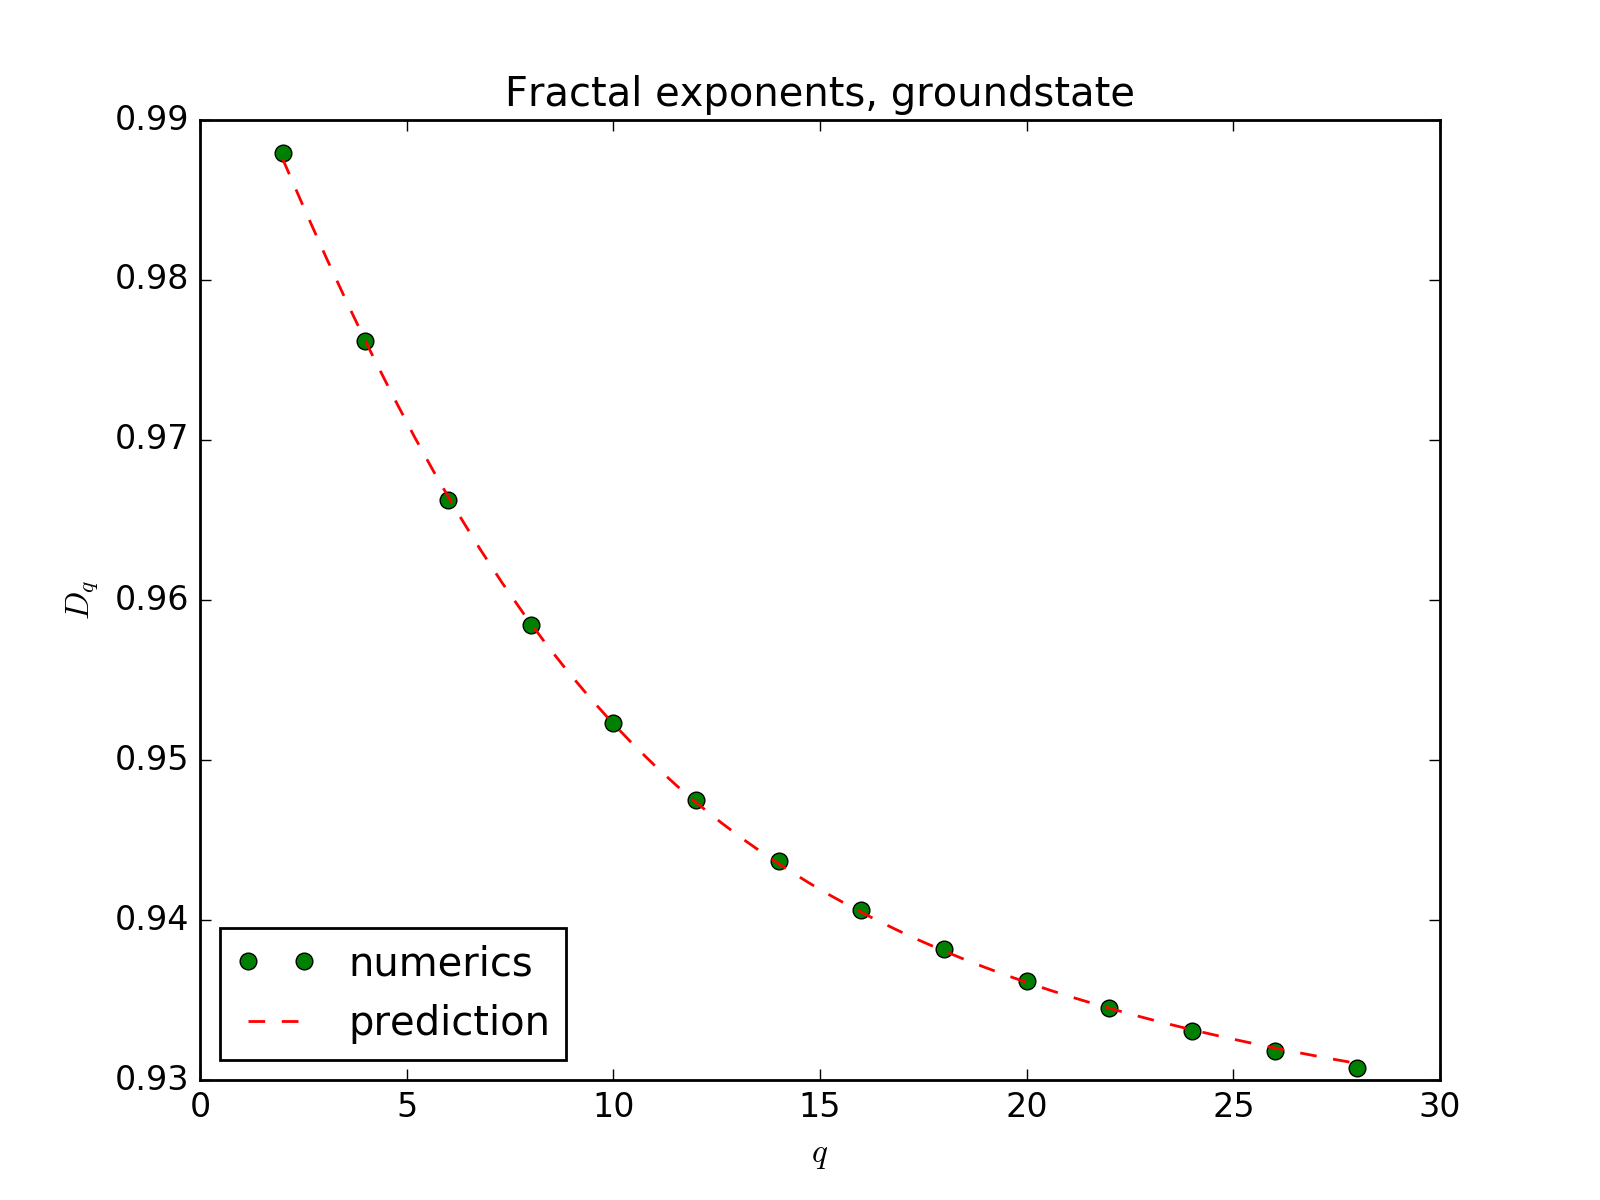
\includegraphics[scale=.4]{img/fractal_exponents_groundstate.png}
\>
\<{7cm}
\[
	t \sum_{n \in V(m)} \psi_n + (t-1)z_m \psi_m = E \psi_m
\]
\centering
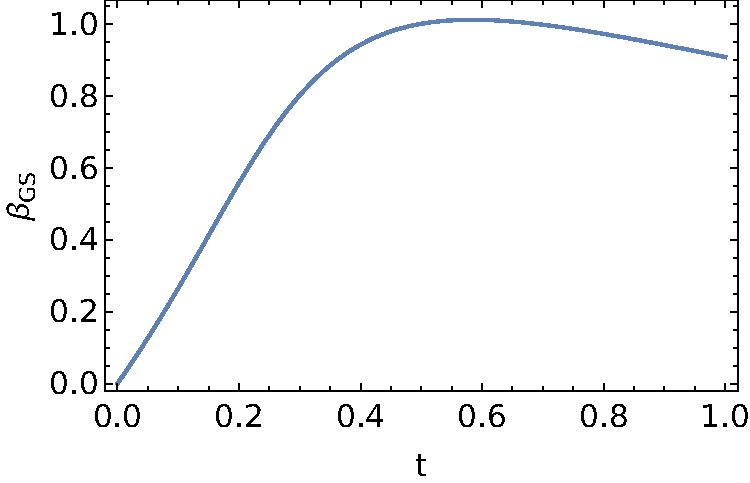
\includegraphics[scale=.6]{img/beta_t.pdf}
\[
	\psi_m = C_m \beta^{h(m)}
\]
\>
\end{columns}
\end{frame}

\end{document}